
\documentclass[a4paper,12pt]{article}

\usepackage[utf8]{inputenc}

\usepackage{listings}
\usepackage[table]{xcolor}
\usepackage{graphicx}
\usepackage{multirow}
\usepackage{tabularx}
\usepackage{pgf-umlcd}

\usepackage[toc,page]{appendix}
\usepackage{upgreek}

\renewcommand{\umltextcolor }{black}
\renewcommand{\umlfillcolor }{white}
\renewcommand{\umldrawcolor }{black}

\graphicspath{{/Users/tom/Documents/Programmieren/ChemBox/Documentation/Images/}}
\lstset{inputpath=/Users/tom/Documents/Programmieren/ChemBox}

\usepackage{algpseudocode}
\usepackage{algorithm}

% Redefine the keywords to use the new command
\algrenewcommand\algorithmicif{\textbf{IF}}
\algrenewcommand\algorithmicthen{\textbf{THEN}}
\algrenewcommand\algorithmicelse{\textbf{ELSE}}
\algrenewcommand\algorithmicend{\textbf{END}}
\algrenewcommand\algorithmicfor{\textbf{FOR}}
\algrenewcommand\algorithmicdo{\textbf{DO}}
\algrenewcommand\algorithmicwhile{\textbf{WHILE}}
\algrenewcommand\algorithmicloop{\textbf{LOOP}}
\algrenewcommand\algorithmicrepeat{\textbf{REPEAT}}
\algrenewcommand\algorithmicuntil{\textbf{UNTIL}}
\algrenewcommand\algorithmicreturn{\textbf{RETURN}}
\algrenewcommand\algorithmicfunction{\textbf{SUBROUTINE}}

\usepackage{tikz}
\usetikzlibrary{shapes.geometric, arrows}

\tikzstyle{startstop} = [rectangle, rounded corners, minimum width=3cm, minimum height=1cm,text centered, draw=black, fill=red!30]
\tikzstyle{io} = [trapezium, trapezium left angle=70, trapezium right angle=110, minimum width=3cm, minimum height=1cm, text centered, draw=black, fill=blue!30]
\tikzstyle{process} = [rectangle, minimum width=3cm, minimum height=1cm, text centered, draw=black, fill=orange!30]
\tikzstyle{decision} = [diamond, minimum width=3cm, minimum height=1cm, text centered, draw=black, fill=green!30]
\tikzstyle{arrow} = [thick,->,>=stealth]

\lstdefinestyle{mystyle}{
    backgroundcolor=\color{backcolour},   
    commentstyle=\color{codegreen},
    keywordstyle=\color{magenta},
    numberstyle=\tiny\color{codegray},
    stringstyle=\color{codepurple},
    basicstyle=\fontsize{8}{10}\ttfamily,
    breakatwhitespace=false,         
    breaklines=true,                 
    captionpos=b,                    
    keepspaces=true,                 
    numbers=left,                    
    numbersep=5pt,                  
    showspaces=false,                
    showstringspaces=false,
    showtabs=false,                  
    tabsize=2,
    frame=single,
}

\lstset{style=mystyle}


\definecolor{codegreen}{rgb}{0,0.6,0}
\definecolor{codegray}{rgb}{0.5,0.5,0.5}
\definecolor{codepurple}{rgb}{0.58,0,0.82}
\definecolor{backcolour}{rgb}{1,1,1}

\title{ChemBox Project Documentation}
\author{Tom Schneider}

\begin{document}
\begin{titlepage}
    \begin{center}
        \vspace*{1cm}
        
        \huge ChemBox Project Documentation
        
        \vspace{1cm}
        
        \Large Tom Schneider
        
        \vfill
        
        \textbf{Date:} \today \\
        
        \vspace{1cm}
        
        \textbf{Centre Number:} 29065 \\
        \textbf{Candidate Number:} 7638 \\
        
        \vspace{1cm}
        
        \textbf{Ellesmere College}
        
    \end{center}
\end{titlepage}

\tableofcontents

\pagebreak

\section{Analysis}

\subsection{Introduction}

Technology gives us the benefits of saving time and doing work more efficiently. The use of software and technology in chemistry does not only help increase accuracy and decrease human error, but also reduces the time spent performing repetitive tasks by hand. ChemBox is a software project with the aim of creating an interactive, user-friendly, and intuitive toolbox for automating and simplifying complex and repetitive tasks that come up on a daily basis for students, educators and professionals in the field of chemistry. The application features a range of different tools that should help chemists work more efficiently and carry out their work more accurately. ChemBox is split into three distinct modules with different functionalities.\\
\linebreak
The first module is the "ChemCalculator". The aim of this part of the program is to help the user carry out calculations by filling in equations and formulae. Although substituting numbers into predefined equations is a rather trivial task, it leaves a lot of room for human error when it comes to things like converting between units or applying mathematical laws correctly. This module should help the user with the most important and at the same time most trivial tasks in chemistry.\\
\linebreak
The second module, "ChemBalancer", is for balancing chemical equations, as the name already suggests. Chemical equations come up in every lab experiment, calculation, or research problem. While balancing short equations made up of very few different elements is arguably a rather easy task, it can get quite tricky when you have to work with a large number of different elements, complex ions or just very long equations. Making just a tiny mistake when balancing an important equation can cause a big setback as it can take long to find small errors like mixing up a 2 with a 3.\\
\linebreak
The third and last module is the "ChemEditor". Visualising molecular structures can play a vital role in understanding a substances chemical properties or understanding interactions with other substances. Drawing molecules out by hand is pretty straight forward. It is knowing when a bond is valid and which atoms bond together and which don't that is the tricky part. Having a tool that can help you make sure the chemical molecule you want to draw can even exist, can be a great help not only for beginner level chemists but also for more experienced chemists.

\newpage

\subsection{Prospective Users}

Chembox will provide valuable tools to a diverse user base, spanning from students to professional chemists. The intuitive and straight forward design will allow users with varying backgrounds and degrees to use ChemBox for their own specific needs.\\
In the early stage, the main users of this system will be pupils and staff attending Ellesmere College, but it could be a goal to make the software available open source to anyone online.\\
Engaging with pupils at the college during the early stages allows for a valuable user feedback loop. This direct interaction with the user group will provide insights into the software's usability, identify potential improvements, and address any specific requirements that may arise within the college context.

\subsubsection{Interview with Oliver Covill - Future User}

To get an independent opinion on the topic when it comes to important features and future design of the system, I have interviewed Oliver Covill, a fellow A-Level chemistry student at Ellesmere College.\\

Q: What are the benefits of performing the tasks manually and by hand?
\linebreak

Oliver: Learning the process of the calculation and what is required for them and why we use them. Doing every step of the task by hand, be it calculating something or balancing an equation gives you a better feeling for it and teaches you the necessary foundations you need.\\
\linebreak

Q: What are the drawbacks of using the current system (by hand/without software)?
\linebreak

Oliver: Longer questions that require multiple equations and rearranging them can be quite tedious at times. Also, checking every calculation performed by hand can be very time consuming. Balancing long equations can sometimes be near impossible or might require multiple lines of working out, to get the right balanced equation, especially if you don't instantly notice a mistake you have made.\\

\newpage
Q: What are the most common tasks in chemistry that could be computed, and which features would be most important to you?\\
\linebreak

Oliver: Definitely a lot of the basic mole like calculations. Also having the ability to do PV=nRT calculations or having a Gibbs Free Energy calculator would be great. The most important Feature for me would be a chemical equation balancer, which is especially important for long and complex equations.


\subsection{Specific Objectives}

Through being an A-Level Chemistry student myself, I have learned a lot about using chemical equations and performing calculations as well as balancing chemical equations and visualising chemical substances and molecules. I was able to identify a number of calculations that processes that come up on a regular basis and divide them into non-negotiable and nice-to-have objectives.

\subsubsection{Chemical Equations and Calculations - ChemCalculator}

The first module of the program is for performing  calculations which are based on chemical formulae.
Where appropriate the program should allow the user to choose from a range of different units for each calculation, so the user doesn't have to calculate the conversions like the one from $cm^{3}$ to $dm^{3}$ for example.\\
\linebreak
Required functionalities:\\
\linebreak

\begin{enumerate}

\item Standard moles calculation:
\[moles=\frac{mass}{molar\: mass}\]

\item Calculation to find the concentration:
\[concentration=\frac{moles}{volume}\]

\newpage

\item Avogadro's number calculations. The user should be able to give several inputs, including mass, moles, molecular weight and the number of atoms. After giving two independent inputs, the program should be able to calculate the rest of the values using Avogadro's number.\\
The equation the calculator will be based on is:
\[number\: of\: atoms = Avogadro's\: number \times moles\]
This should be paired with a mole calculator for the possibility use the following formula:
\[number\: of\: atoms = Avogadro's\: number \times \frac{mass}{molar\: mass}\]

\item Gibbs Free Energy calculation:
\[{\Delta}G = {\Delta}H - T{\Delta}S\]
\begin{quote}
(${\Delta}$G = Gibbs Free Energy) (${\Delta}$H = enthalpy)\\
(T = temperature) (${\Delta}$S = entropy)
\end{quote}

\item Calculation for the Specific Heat Capacity and Enthalpy changes:
\[q = mc {\Delta} T\]
\begin{quote}
(q = energy change) (m = mass) (c = specific heat capacity) (${\Delta}$T = temperature change)
\end{quote}

\item Equilibrium Constant calculation for a reversible reaction:
\[a[A] + b[B] \rightleftharpoons c[C] + d[D]\]
\[K_{C} = \frac{[C]^{c}[D]^{d}}{[A]^{a}[B]^{b}}\]
\begin{quote}
($K_{C}$ = Equilibrium Constant) (Upper case letter = Concentration) (Lower case letter = Moles in Equation)
\end{quote}

\item Rate Equation and Rate constant calculation:
\[Rate = k[A]^{m}[B]^{n}\]

\item Ideal Gas Law calculation:
\[PV = nRT\]
\begin{quote}
(P = Pressure, V = Volume, n = Number of moles, R = Gas constant, T = Temperature)
\end{quote}

\end{enumerate}

\newpage

Non-essential objectives:
\begin{enumerate}
\item Acid calculations - pH and $[H^{+}]$
\[pH = -log[H^{+}]\]
\[[H^{+}] = 10^{-pH}\]

\item Acid dissociation constants $K_{a}$ and $pK_{a}$
\[K_{a} = \frac{[H^{+}][A^{-}]}{[HA]}\]
\[pK_{a} = -logK_{a}\]
\[K_{a} = 10^{-pK_{a}}\]

\item Atom Economy calculation:
\[Atom\: Economy = \frac{Mr\: of\: desired\: product}{Sum\: of\: Mr\: of\: all\: reactants}\times 100\]

\item Percentage Yield calculation:
\[\%Yield = \frac{Actual\: yield}{Theoretical\: yield} \times 100\]

\end{enumerate}

\newpage

\subsubsection{Chemical Equation Balancer - ChemBalancer}

A substantial part of the project will be the ChemBalancer which will be the module that balances chemical equations. This system must be able to take complex unbalanced equations and convert them into a balanced version.\\
It must be able to handle subscript numbers, brackets, and complex ions.

\subsubsection{Visualisation of Chemical Molecules - ChemEditor}

The third part of the program will be the ChemEditor module, which can be used for visualising the structures of chemical molecules. This module will require a user-friendly and easy to use interface, with the main focus on the canvas. The user should have the option to choose from a range of different elements what he wants to add to the canvas. In a tool bar, the user should also be able to choose the bond order (single, double, triple) and the charge on each atom. When clicking on an atom, there should be an option to add a bond to another atom or delete the atom.\\
When the user constructs their molecules, ChemEditor will have to conduct real-time checks to ensure that atoms do not exceed their valence electrons and that it is chemically possible to have a molecule with the given structure. \\
The required objectives for this module are:\\

\begin{enumerate}

\item Tool bar:\\
In the tool bar on the top end of the application, there must be a list of buttons for choosing the element, which must include the most common elements (Carbon, Hydrogen, Sulphur, Chlorine, etc.). There also has to be the option to choose the bond order (single, double or triple bond). Another essential option in form of buttons should be removing atoms and bonds as well as being able to safe the drawn structures as a document.\\
A possible non-essential enhancement would be getting extra information about atoms upon highlighting as well as getting information like the molar mass and the empirical formula of a molecule after highlighting.
\item Canvas:\\
The canvas is the area in which the user can draw their molecules. There are several features that must be included here.\\
	\begin{enumerate}
	\item The user must be able to draw atoms by clicking on the canvas.
	\item Upon selecting an existing atom on the canvas, depending on the chosen action type, the user should have different options:
		\begin{enumerate}
		\item When the chosen action type is "Draw", a number of greyed out atoms and bonds to those atoms should be drawn, out of which the user can choose where he wants to place his next atom.
		\item When the chosen action type is "Bond", the program should draw a bond from the selected atom to every existing atom on the canvas, with which a bond would be possible. The colour of those bonds needs to be different to the colour of the actual existing 		bonds, to avoid confusion.
		\end{enumerate}
	\end{enumerate}
\end{enumerate}

\subsection{Current and Proposed Systems}

The current standard is to work out chemical equations or draw molecules on paper. This might make sense for simple equations or small molecules, but it gets less efficient and more difficult as complexity increases. Although there are some software solutions for very specific tasks, there isn't one intuitive and easy to use application that combines the different tasks in one place.\\
\linebreak
Naturally, drawing molecules with pen and paper feels best and is the preferred choice by most people. This project is not here to replace that, it should merely pose as a help for chemists when working certain things out.

\newpage

\section{Documented Design}

\subsection{Introduction to the Documented Design}

In this section, I will outline the decisions, that have outlined the development of the ChemBox project and explain the programming techniques used to implement certain algorithms and structures.\\
The program is written in python, with the aim of using as little external frameworks and dependencies as possible, and therefore creating most of this project from scratch. For the GUI implementation, I chose to use the PyQt6 framework, which is a powerful tool for creating GUI applications in python.\\

\subsection{Project Hierarchy}

As mentioned in the analysis part of this document, the project is separated into three standalone modules which are merged in the main class of the program, ChemBox.

\begin{figure} [h]
	\centering
	\includegraphics[scale=0.4]{base_hierarchy}
	\caption{Program Hierarchy chart}
	\label{fig:tabs_mockup}
\end{figure}

I will explain the hierarchy and program flow of the system, beginning with the ChemCalculator module.
\newpage

\subsection{Structure of the GUI}

The ChemBox class is the heart of the program, the point where all the different components are merged to create one complete application. To give a better understanding of the system, I will explain how I composed the GUI and what each major component does. The ChemBox class contains only the constructor method, in which the layout of the graphical user interface is specified. The constructor defines the dimensions, the title and geometry of the window and then creates an instance of the TabBar class, which will act as the central widget of the program. Next, an instance of each of the three big components of the project, ChemCalculator, ChemBalancer and ChemEditor is created, and allocated to a separate tab of the tab bar (Listing \ref{lst:chembox_snippet}: lines 18 - 25).

\begin{lstlisting}[language=Python, caption=Code snippet of ChemBox class, label={lst:chembox_snippet}]
class ChemBox(QMainWindow):
    def __init__(self):
        super().__init__()

        # set window properties
        self.__left = 300
        self.__top = 300
        self.__width = 1280
        self.__height = 720
        self.__title = "ChemBox"
        self.setWindowTitle(self.__title)
        self.setGeometry(self.__left, self.__top, self.__width, self.__height)
        self.setFixedSize(self.__width, self.__height)

        self.tab_bar = TabBar()
        self.setCentralWidget(self.tab_bar)

        self.chem_calculator = ChemCalculator()
        self.tab_bar.tab1.setLayout(self.chem_calculator.main_layout)

        self.chem_balancer = ChemBalancer()
        self.tab_bar.tab2.setLayout(self.chem_balancer.balancer_layout)

        self.chem_editor = ChemEditor()
        self.tab_bar.tab3.setLayout(self.chem_editor.editor_layout)
\end{lstlisting}

\newpage
The tab bar is used as the main widget of the program at all times, as it controls the navigation between modules.
The goal was to achieve a design like the one illustrated in Figure \ref{fig:tabs_mockup}, where 1, 2 and 3 in the small boxes at the top of the screen represent buttons in the tab bar for the three major modules of the ChemBox.

\begin{figure} [h]
	\centering
	\includegraphics[scale=0.4]{tabs_mockup}
	\caption{Mockup drawing of tab bar}
	\label{fig:tabs_mockup}
\end{figure}

The ChemCalculator module is the only part of the project with a special implementation of the user interface, which needs explanation.\\

When developing the ChemCalculator module, the first issue I encountered was how I would create a layout that would work for multiple separate sub-calculators. I had three different possible systems for displaying the module. The first option was creating a sidebar, where the user can choose the exact calculator, they were looking for, which is then displayed on the screen. The second option was very similar, but with an additional tab bar at the top or bottom of the screen. This solution is not very aesthetically pleasing and could cause confusion with the actual tab bar that allows the user to switch between the three main modules. The third option was putting every calculator on the same page, each in its own area, clearly separated from the others, and make the window scrollable. I decided against this option, as this design could have gotten very messy. Therefore, I decided to create a sidebar for the ChemCalculator. \\
As there is no built-in sidebar widget in PyQt6, I have designed my own way of creating one. I did so by using the QTabWidget, which I also used for the tab bar, but not display it. I was able to benefit from the already existing widget, for the switching between calculators, and use buttons placed on the left side of the screen as a replacement for an actual sidebar. The buttons connect to a method, which changes the current index of the tab widget to the according number of the calculator, which updates the page that is displayed. This is illustrated in the following code snippet (Listing \ref{lst:chemcalculator_example}), which only includes the example on a single button, for better readability of this document.

\begin{lstlisting}[language=Python, caption=Example of ChemCalculator implementation, label={lst:chemcalculator_example}]
class ChemCalculator(QWidget):
    def __init__(self):
        super(QWidget, self).__init__()

        self.side_bar_layout = QVBoxLayout()

        self.gibbs_calc = GibbsFreeEnergyCalculator()

        # Create buttons
        self.gibbs_free_energy_tab_button = QPushButton("Gibbs Free Energy Calculator")

        self.gibbs_free_energy_tab_button.clicked.connect(self.gibbs_free_energy_action)

        # Create tabs
        self.gibbs_free_energy_tab = QWidget()

        # Initialise gibbs free energy calculator
        self.gibbs_free_energy_tab.setLayout(self.gibbs_calc.layout)
        
        # Add buttons to sidebar layout
        self.side_bar_layout.addWidget(self.gibbs_free_energy_tab_button)

        self.side_bar_widget = QWidget()
        self.side_bar_widget.setLayout(self.side_bar_layout)

        self.page_widget = QTabWidget()

        self.page_widget.addTab(self.gibbs_free_energy_tab, "")
        
        self.page_widget.setCurrentIndex(0)
        self.page_widget.setStyleSheet('''QTabBar::tab{
        width: 0; 
        height: 0; 
        margin: 0; 
        padding: 0; 
        border: none;
        }''')

        self.main_layout = QHBoxLayout()
        self.main_layout.addWidget(self.side_bar_widget)
        self.main_layout.addWidget(self.page_widget)

        self.main_widget = QWidget()
        self.main_widget.setLayout(self.main_layout)

    # Define actions for each button
    def gibbs_free_energy_action(self):
        self.page_widget.setCurrentIndex(5)

\end{lstlisting}

\subsection{Algorithm Design for ChemCalculator}

Essential for most individual calculators in the ChemCalculator module will be an algorithm to determine which of the input options the user left blank. In general, the user interface will always consist of a number of inputs, implemented as QLineEdit's, where the blank ones are the ones that our program will calculate.\\
The algorithm will have to take a list of inputs as a parameter and use iteration to determine the blank one.

\begin{algorithm}
\caption{Algorithm to find empty input}\label{alg:fing_empty_input}
\begin{algorithmic}
\State $ input\_list \gets []$
\State $ count \gets 0$
\State $ empty\_input \gets NONE$
\For{$i \gets 0\ to\ Len(input$\_$list)$}
\If{$ input\_list[i]\ is\ empty$}
	\State $ count \gets count\ $+$\ 1$
	\State $ empty\_input \gets input\_list[i]$
\EndIf
\EndFor
\If{$ count = 1 $}
	\State $ RETURN\ count$
\EndIf
\end{algorithmic}
\end{algorithm}

\newpage

\subsection{Algorithm Design for ChemBalancer}

Figure \ref{fig:balance_flow} includes my initial attempt at visualising how an equation balancer could work. My first version of this module worked on a very similar system, although I struggled with finding a method of consistently balancing the equations after splitting them into their smallest possible components. 

\begin{figure} [h]
	\centering
	\includegraphics[scale=0.4]{balance_flow}
	\caption{Initial flowchart for balancer}
	\label{fig:balance_flow}
\end{figure}

The following code blocks contains the code of my initial, failed, attempt at the balancer.

\begin{lstlisting}[language=Python, caption=Method for splitting equation into components, label={lst:split_equation}]
def splitEquation(self):
        self.equationSplit = self.equationInput.text().split(" = ")
        self.reactants = self.equationSplit[0]
        try:
            self.products = self.equationSplit[1]
        except IndexError:
            print("Wrong user input")
        self.reactantComponents = self.reactants.split(" + ")
        self.productComponents = self.products.split(" + ")
\end{lstlisting}

The splitEquation method uses string manipulation to extract the individual molecules of the equation and store them in separate lists for reactants and products.\\
After finding the individual molecules in the equation, the parseComponent method is called to get the elements used in the molecules, and the amount of them. This is done through if statements, as there is only a limited number of different possibilities. The longest element symbol consists of three letters, where the first letter of every atom is always capitalised, and the following ones are not. The subscript number (number of atoms or element in a given molecule) can be found easily, as numbers within molecules always belong to the preceding element (H2O - the 2 belongs to the hydrogen). Individual elements are found by checking for capital letters. An element starts with a capital letter and ends at the next capital letter, which is where the next element starts. The same techniques were used to find brackets.

\begin{lstlisting}[language=Python, caption=parseComponent method for finding elements, label={lst:parsecomponent}]
def parseComponent(self, component, countsDict, totalDict):
        # Check for coefficient
        try:
            if component[0] in self.integers:
                try:
                    if component[0 + 1] in self.integers:
                        try:
                            if component[0 + 2] in self.integers:
                                coefficient = int(component[0: 0 + 3])
                            else:
                                coefficient = int(component[0: 0 + 2])
                        except IndexError:
                            coefficient = int(component[0: 0 + 2])
                    else:
                        coefficient = int(component[0])
                except IndexError:
                    coefficient = int(component[0])
            else:
                coefficient = 1
            for i in range(len(component)):
                try:
                    openBracket = component.find("(")
                    closedBracket = component.find(")")
                except IndexError:
                    continue
                try:
                    if component[i].isupper() and component[i - 1] != "(":
                        try:
                            if component[i + 1].islower():
                                try:
                                    if component[i + 2].islower():
                                        element = component[i:(i + 3)]
                                        if openBracket < i < closedBracket:
                                            subCoefficient = self.getSubCoefficient(component)
                                        else:
                                            subCoefficient = 1

                                        # Check for subscript
                                        try:
                                            if component[i + 3] in self.integers:
                                                try:
                                                    if component[i + 4] in self.integers:
                                                        try:
                                                            if component[i + 5] in self.integers:
                                                                subscript = int(component[(i + 3): (i + 6)])
                                                            else:
                                                                subscript = int(component[(i + 3): (i + 5)])
                                                        except IndexError:
                                                            subscript = int(component[(i + 3): (i + 5)])
                                                    else:
                                                        subscript = int(component[i + 3])
                                                except IndexError:
                                                    subscript = int(component[i + 3])
                                            else:
                                                subscript = 1
                                        except IndexError:
                                            subscript = 1
                                    else:
                                        element = component[i:(i + 2)]

                                        if openBracket < i < closedBracket:
                                            subCoefficient = self.getSubCoefficient(component)
                                        else:
                                            subCoefficient = 1

                                        # Check for subscript
                                        try:
                                            if component[i + 2] in self.integers:
                                                try:
                                                    if component[i + 3] in self.integers:
                                                        try:
                                                            if component[i + 4] in self.integers:
                                                                subscript = int(component[(i + 2): (i + 5)])
                                                        except IndexError:
                                                            subscript = int(component[(i + 2): (i + 4)])
                                                except IndexError:
                                                    subscript = int(component[i + 2])
                                            else:
                                                subscript = 1
                                        except IndexError:
                                            subscript = 1
                                except IndexError:
                                    element = component[i:(i + 2)]
                                    if openBracket < i < closedBracket:
                                        subCoefficient = self.getSubCoefficient(component)
                                    else:
                                        subCoefficient = 1
                            else:
                                element = component[i]
                                if openBracket < i < closedBracket:
                                    subCoefficient = self.getSubCoefficient(component)
                                else:
                                    subCoefficient = 1
                                try:
                                    # Check for subscript
                                    if component[i + 1] in self.integers:
                                        try:
                                            if component[i + 2] in self.integers:
                                                try:
                                                    if component[i + 3] in self.integers:
                                                        subscript = int(component[i + 1: i + 4])
                                                except IndexError:
                                                    subscript = int(component[i + 1: i + 3])
                                            else:
                                                subscript = int(component[i + 1])
                                        except IndexError:
                                            subscript = int(component[i + 1])
                                    else:
                                        subscript = 1
                                except IndexError:
                                    subscript = 1
                        except IndexError:
                            element = component[i]

                            if openBracket < i < closedBracket:
                                subCoefficient = self.getSubCoefficient(component)
                            else:
                                subCoefficient = 1

                            try:
                                # Check for subscript
                                if component[i + 1] in self.integers:
                                    try:
                                        if component[i + 2] in self.integers:
                                            try:
                                                if component[i + 3] in self.integers:
                                                    subscript = int(component[i + 1: i + 4])
                                            except IndexError:
                                                subscript = int(component[i + 1: i + 3])
                                        else:
                                            subscript = int(component[i + 1])
                                    except IndexError:
                                        subscript = int(component[i + 1])
                                else:
                                    subscript = 1
                            except IndexError:
                                subscript = 1
                        try:
                            if element in countsDict:
                                countsDict[element] = int(countsDict[element]) + subscript * coefficient * subCoefficient
                            else:
                                countsDict[element] = subscript * coefficient * subCoefficient

                            if element in totalDict:
                                totalDict[element] = int(totalDict[element]) + subscript * coefficient * subCoefficient
                            else:
                                totalDict[element] = subscript * coefficient * subCoefficient
                        except UnboundLocalError:
                            continue

                    # Check for brackets / complex ion in equation
                    elif component[i] == "(":
                        try:
                            if component[i + 2] == ")":
                                element = component[i + 1]
                                try:
                                    if component[i + 3] in self.integers:
                                        try:
                                            if component[i + 4] in self.integers:
                                                try:
                                                    if component[i + 5] in self.integers:
                                                        subscript = int(component[(i + 3): (i + 6)])
                                                    else:
                                                        subscript = int(component[(i + 3): (i + 5)])
                                                except IndexError:
                                                    subscript = int(component[(i + 3): (i + 5)])
                                            else:
                                                subscript = int(component[(i + 3): (i + 4)])
                                        except IndexError:
                                            subscript = int(component[i + 3])
                                    else:
                                        subscript = 1
                                except IndexError:
                                    subscript = 1
                            elif component[i + 1].isupper():
                                if component[i + 2].islower():
                                    try:
                                        if component[i + 3].islower():
                                            element = component[(i + 1): (i + 4)]

                                            # Check for subscript within brackets
                                            try:
                                                if component[i + 4] in self.integers:
                                                    try:
                                                        if component[i + 5] in self.integers:
                                                            try:
                                                                if component[i + 6] in self.integers:
                                                                    subscript = int(component[(i + 4): (i + 7)])
                                                                else:
                                                                    subscript = int(component[(i + 4): (i + 6)])
                                                            except IndexError:
                                                                subscript = int(component[(i + 4): (i + 6)])
                                                        else:
                                                            subscript = int(component[i + 4])
                                                    except IndexError:
                                                        subscript = int(component[i + 4])
                                                else:
                                                    subscript = 1
                                            except IndexError:
                                                subscript = 1

                                            # Find subscript coefficient of complex ion
                                            subCoefficient = self.getSubCoefficient(component)
                                        else:
                                            element = component[(i + 1): (i + 3)]

                                            # Check for subscript within brackets
                                            try:
                                                if component[i + 3] in self.integers:
                                                    try:
                                                        if component[i + 4] in self.integers:
                                                            try:
                                                                if component[i + 5] in self.integers:
                                                                    subscript = int(component[(i + 3): (i + 6)])
                                                                else:
                                                                    subscript = int(component[(i + 3): (i + 5)])
                                                            except IndexError:
                                                                subscript = int(component[(i + 3): (i + 5)])
                                                    except IndexError:
                                                        subscript = int(component[i + 3])
                                                else:
                                                    subscript = 1
                                            except IndexError:
                                                subscript = 1

                                            # Find subscript coefficient of complex ion
                                            subCoefficient = self.getSubCoefficient(component)
                                    except IndexError:
                                        element = component[(i + 1): (i + 3)]

                                        # Check for subscript within brackets
                                        try:
                                            if component[i + 3] in self.integers:
                                                try:
                                                    if component[i + 4] in self.integers:
                                                        try:
                                                            if component[i + 5] in self.integers:
                                                                subscript = int(component[(i + 3): (i + 6)])
                                                            else:
                                                                subscript = int(component[(i + 3): (i + 5)])
                                                        except IndexError:
                                                            subscript = int(component[(i + 3): (i + 5)])
                                                except IndexError:
                                                    subscript = int(component[i + 3])
                                            else:
                                                subscript = 1
                                        except IndexError:
                                            subscript = 1

                                        # Find subscript coefficient of complex ion
                                        subCoefficient = self.getSubCoefficient(component)
                                else:
                                    element = component[i + 1]

                                    # Check for subscript within brackets
                                    try:
                                        if component[i + 2] in self.integers:
                                            try:
                                                if component[i + 3] in self.integers:
                                                    try:
                                                        if component[i + 4] in self.integers:
                                                            subscript = int(component[(i + 2): (i + 5)])
                                                        else:
                                                            subscript = int(component[(i + 2): (i + 4)])
                                                    except IndexError:
                                                        subscript = int(component[(i + 2): (i + 4)])
                                            except IndexError:
                                                subscript = int(component[i + 2])
                                        else:
                                            subscript = 1
                                    except IndexError:
                                        subscript = 1

                                    # Find subscript coefficient of complex ion
                                    subCoefficient = self.getSubCoefficient(component)
                        except IndexError:
                            print("wrong user input ")
                        try:
                            if element in countsDict:
                                countsDict[element] += subscript * subCoefficient * coefficient
                            else:
                                countsDict[element] = subscript * subCoefficient * coefficient
                            if element in totalDict:
                                totalDict[element] += subscript * subCoefficient * coefficient
                            else:
                                totalDict[element] = subscript * subCoefficient * coefficient
                        except UnboundLocalError:
                            continue
                    else:
                        continue
                except IndexError:
                	continue
        except IndexError:
            None
\end{lstlisting}

Although this code is overly complicated, it worked most of the times for basic or intermediate level equations.\\
The main problem this version of the balancer ran into, was the actual balancing of the equations. The version uses a loop to attempt balancing, where copies of the left- and right-hand side components are created together with dictionaries to track the total count of elements. Each component then gets a randomly generated coefficient between 1 and 10, and the loop continues until the count on the left side equals the count on the right side. Once a balanced equation is found, the coefficients are normalised to their smallest integer values using the greatest common divisor (GCD) The balanced equation is then put back together and returned to the user.\\

\begin{lstlisting}[language=Python, caption=balance method, label={lst:balance_method}]
def balance(self):
        if self.balanced:
            equation = str()
            for dictionary in self.left:
                compound = str()
                for element in dictionary:
                    compound += element
                    if dictionary[element] > 1:
                        compound += str(dictionary[element])
                equation += compound
                equation += " + "
            equation = equation[:len(equation) - 3] + " = "
            for dictionary in self.right:
                compound = str()
                for element in dictionary:
                    compound += element
                    if dictionary[element] > 1:
                        compound += str(dictionary[element])
                    else:
                        pass
                equation += compound
                equation += " + "
            equation = equation[:len(equation) - 2]
        else:
            while not self.balanced:
                tempLeft = list()
                tempRight = list()
                totalLeft = dict()
                totalRight = dict()

                for item in self.left:
                    newDict = dict()
                    for key in item:
                        newDict[key] = item[key]
                    tempLeft.append(newDict)

                for item in self.right:
                    newDict = dict()
                    for key in item:
                        newDict[key] = item[key]
                    tempRight.append(newDict)

                leftCoefficients = [randint(1, 10) for _ in range(len(tempLeft))]
                rightCoefficients = [randint(1, 10) for _ in range(len(tempRight))]

                for index in range(0, len(leftCoefficients)):
                    for key in tempLeft[index]:
                        tempLeft[index][key] *= leftCoefficients[index]
                        if key not in totalLeft:
                            totalLeft[key] = tempLeft[index][key]
                        else:
                            totalLeft[key] += tempLeft[index][key]
                for index in range(0, len(rightCoefficients)):
                    for key in tempRight[index]:
                        tempRight[index][key] *= rightCoefficients[index]
                        if key not in totalRight:
                            totalRight[key] = tempRight[index][key]
                        else:
                            totalRight[key] += tempRight[index][key]
                self.balanced = True
                for key in totalLeft:
                    if totalLeft[key] != totalRight[key]:
                        self.balanced = False
                    else:
                        continue

            bigTup = tuple(leftCoefficients + rightCoefficients)
            leftCoefficients = list(map(lambda x: int(x / reduce(gcd, bigTup)), leftCoefficients))
            rightCoefficients = list(map(lambda x: int(x / reduce(gcd, bigTup)), rightCoefficients))

            balancedEquation = str()
            for index in range(0, len(self.left)):
                if leftCoefficients[index] != 1:
                    compound = str(leftCoefficients[index])
                else:
                    compound = str()
                for key in self.left[index]:
                    compound += key
                    if self.left[index][key] != 1:
                        compound += str(self.left[index][key])
                balancedEquation += compound
                balancedEquation += " + "
            balancedEquation = balancedEquation[:len(balancedEquation) - 3] + " = "
            for index in range(0, len(self.right)):
                if rightCoefficients[index] != 1:
                    compound = str(rightCoefficients[index])
                else:
                    compound = str()
                for key in self.right[index]:
                    compound += key
                    if self.right[index][key] != 1:
                        compound += str(self.right[index][key])
                balancedEquation += compound
                balancedEquation += " + "
            balancedEquation = balancedEquation[:len(balancedEquation) - 2]
            return self.balancedLabel.setText(f"{balancedEquation}")
\end{lstlisting}

\newpage

This version had a few obvious limitations, it relied on randomly generated coefficients, which is not a very reliable system of finding the correct coefficients. Although the random generation usually provides coefficients, it  may not always produce the most optimal or smallest possible coefficients. The normalisation step using the greatest common divisor ensures that the coefficients are integer multiples of each other, but it does not guarantee the smallest 	possible coefficients. If a balanced equation cannot be found with the randomly generated coefficients, there is also a possibility of infinite looping.

\begin{figure} [h]
	\centering
	\includegraphics[scale=0.5]{initial_balance_test}
	\caption{Initial balancer test}
	\label{fig:initial_balance_test}
\end{figure}

The test in Figure \ref{fig:initial_balance_test} shows, that the system works (at least for simple equations). Just the simple addition of two carbon atoms and four hydrogen atoms to get the equation $ C2H6 + O2 = CO2 + H2O$ is already too much for the system, as this will end in an infinite loop. This loop can be prevented by increasing the range of possibilities for the randomly generated integers (for example from between 1 and 10 to between 1 and 100) but this means there is always a limit to what is possible for the balancer. Figure \ref{fig:second_balance_test} shows the state of the program after trying to balance the equation with the original range of one to 10. The program in the figure is in the state of an infinite loop.

\begin{figure} [h]
	\centering
	\includegraphics[scale=0.5]{initial_balance_test2}
	\caption{Initial balancer test No. 2}
	\label{fig:second_balance_test}
\end{figure}

\newpage

Whilst researching for better ways to implement a chemical equation balancer in python, I came across regular expressions, which around that same time, we also covered in our A-Level Computer Science lessons. Knowing about regular expressions helped me significantly improve the effectiveness of my balancer when it comes to extracting individual elements and their amount from the equation. In my search for the best possible way to do so, I wrote several algorithms, which extend each other perfectly, to finish the job together.\\
This algorithm (Algorithm \ref{alg:new_split_equation}) takes the full equation as a parameter from the user input and removes any white spaces from it. It then splits it up into separate reactants and products, and lastly, it extracts the individual reagents within the reactants and products.
\begin{algorithm}
\caption{Algorithm to split equation}\label{alg:new_split_equation}
\begin{algorithmic}
\Function{$ split\_equation$}{$ $}
\State $ stripped\_equation \gets USERINPUT$
\State $ stripped\_equation \gets stripped\_equation.STRIP(" ")$
\State $ equation\_split \gets stripped\_equation.SPLIT("=")$
\State $ reactants \gets equation\_split[0].SPLIT("+")$
\State $ products \gets equation\_split[1].SPLIT("+")$
\EndFunction
\end{algorithmic}
\end{algorithm}

This second algorithm(Algorithm \ref{alg:find_reagents}), which I designed for the task mentioned above, uses regular expressions, to identify separate reagents within a chemical compound by identifying brackets. The goal is to split up compounds like $ CuNO3)2$ into $ ["Cu",\ "(NO3)2"]$, where $Cu$ and $(NO3)2$ are two separate entries in the list. The method then iterates over each reagent, and checks if it starts with an opening bracket. If it does, this indicates, that there is a chemical compound enclosed in the brackets. It extracts the inner compound and the subscript ($ (OH)2$ indicates that the $(OH)$ group exists twice), and then passes these two variables as parameters to the "find\_elements" method, along with the "index" and "side" parameters.

\begin{algorithm}
\footnotesize
\caption{Algorithm to find reagents}\label{alg:find_reagents}
\begin{algorithmic}
\Function{$find\_reagents$}{$compound,\ index,\ side$}
\State $ reagents \gets SPLIT\ compound\ INTO\ reagents\ USING\ REGEX\ PATTERN$
\For{$ reagent\ IN\ reagents$}
\If{$ reagent\ BEGINS\ WITH\ "("$}
	\State $ inner\_compound \gets SUBSTRING(1,\ LEN(reagent))$
	\State $ bracket\_subscript \gets SPLIT\ reagent\ BY\ ")"\ AND\ GET\ SECOND\ PART$
	\If{$ bracket\_subscript\ EXISTS$}
		\State $ bracket\_subscript \gets INT(bracket\_subscript)$
	\Else
		\State $ bracket\_subscript \gets 1$
	\EndIf
	\State $ find\_elements(inner\_compound,\ index,\ bracket\_subscript,\ side)$
\Else
	\State $ bracket\_subscript \gets 1$
	\State $ find\_elements(reagent,\ index,\ bracket\_subscript,\ side)$
\EndIf
\EndFor
\EndFunction
\end{algorithmic}
\end{algorithm}

The next algorithm (Algorithm \ref{alg:find_elements}) uses a regular expression to obtain the elements and associated subscript values. Each extracted element is then stored together with the correlated subscript value as a tuple, inside a list (For example: $Cr2O7$ $\rightarrow$ $[("Cr",\ "2"),\ ("O",\ "7")]$). The algorithm then iterates through each tuple (elements, subscript) in the element\_counts list.
With every iteration, a different subroutine named add\_to\_matrix is called, passing the current element, index, the product of the bracket\_subscript and subscript, and the side argument.

\newpage

\begin{algorithm}
\footnotesize
\caption{Algorithm to find elements}\label{alg:find_elements}
\begin{algorithmic}
\Function{$find\_reagents$}{$reagent,\ index,\ bracket\_subscript,\ side$}
\State $ element\_counts \gets SPLIT\ reagent\ INTO\ element\_counts\ USING\ REGEX\ PATTERN$
\For{$ element,\ subscript\ IN\ element\_counts$}
\If{$ subscript\ DOES\ NOT\ EXIST$}
	\State $ subscript \gets 1$
\Else
	\State $ subscript \gets INT(subscript)$
\EndIf
\State $ add\_to\_matrix(element,\ index,\ bracket\_subscript * subscript,\ side)$
\EndFor
\EndFunction
\end{algorithmic}
\end{algorithm}

While I was conducting my research, I found a neat solution to balancing equations, matrix operations. As we had only covered the rudimentary principles of matrix operations, I chose to use the article \cite{balancing-algorithm} I had found on the internet to get a better understanding of the topic. After getting a grasp of the concept, and after trying out the code in the article, I had found a different way to tackle my problem. I decided not to reinvent the wheel, but to take the already existing algorithm and improve it, so it could be used for practically any tractable equation there is.\\
To address the problem, I decided to record a number of issues and possible improvements for the existing algorithm.

\begin{enumerate}
\item The first issue I had with the algorithm was, that it asked for separate inputs of reactants and products. Luckily, I had already solved this problem with the algorithms illustrated earlier.
\item Another issue the original algorithm had was the lack of structure and modularity. By organising the code in a class based structure, I ensured good readability for the code, as well as making it easier to maintain.
\item The original version had poor input validation and error handling. One common error I got with the early implementation of the algorithm was what I call a nullspace error. The nullspace is a linear subspace that contains a set of vectors that transform to the zero$^{th}$ vector under a given linear transformation: multiplication with the matrix A, represented as $ Ax = 0$.\cite{nullspace} In the context of chemical equations, the nullspace contains the coefficients, that balance the equation.\\
Entering the unbalanced equation $ K4[Fe(SCN)6] + K2Cr2O7 + H2SO4$\\ $ = Fe2(SO4)3 + Cr2(SO4)3 + CO2 + H2O + K2SO4 + KNO3$ resulted in a "nullspace error" (Figure \ref{fig:nullspace_error}). 

\newpage

\begin{figure} [h]
	\centering
	\includegraphics[scale=0.4]{nullspace_error}
	\caption{Nullspace error}
	\label{fig:nullspace_error}
\end{figure}

I managed to neutralise this error by having a more accurate and efficient method of separating out molecules, elements, etc. as shown in Algorithm \ref{alg:find_reagents} and Algorithm \ref{alg:find_elements}, before passing them on to the method that adds the items to the matrix.\\
I also made sure to use pythons built in exception handling to catch any expected and unexpected errors or exceptions.
\end{enumerate}

Using the current working system, inputting the chemical equation mentioned before results in a perfectly balanced equation (Figure \ref{fig:working_balancer}).

\begin{figure} [h]
	\centering
	\includegraphics[scale=0.3]{working_balancer}
	\caption{Balanced equation}
	\label{fig:working_balancer}
\end{figure}

\newpage

\subsection{Algorithm Design for ChemEditor}

My initial attempt at creating the ChemEditor was a mixture of following the plan made in the analysis stage and trying out different things to see what works best.\\
\linebreak
To start my work on this module, I decided to try to identify a number of structures I will have to implement. The ChemEditor can be broken down into a graphical user interface part and a logic part. The GUI section has to consist of two main classes, the "ChemEditor" class, which takes care of displaying all the buttons, the canvas and other parts of the GUI, and the "Canvas" class, which can be further broken down into two main structures, the "paintEvent", which takes care of all the drawing, and the\\ "mousePressEvent", which defines what is supposed to happen after a user's interaction with the interface. The segment taking care of the logic of this module must contain an "Atom" class and a "Bond" class which define certain actions and properties.\\

\subsubsection{ChemEditor Logic}

I first started my work on the logic of the module, where my initial action was to define the Atom class and the Bond class and their associated methods and variables. The Atom class is the blueprint used for every individual atom on the canvas. The Bond class is only used in the bond() method of the Atom class, where a new bond between two atoms is initiated. Each atom can have as many bonds as it has free spaces in its outer shell, while each instance of a bond must always exist of exactly two atoms.

\begin{center}
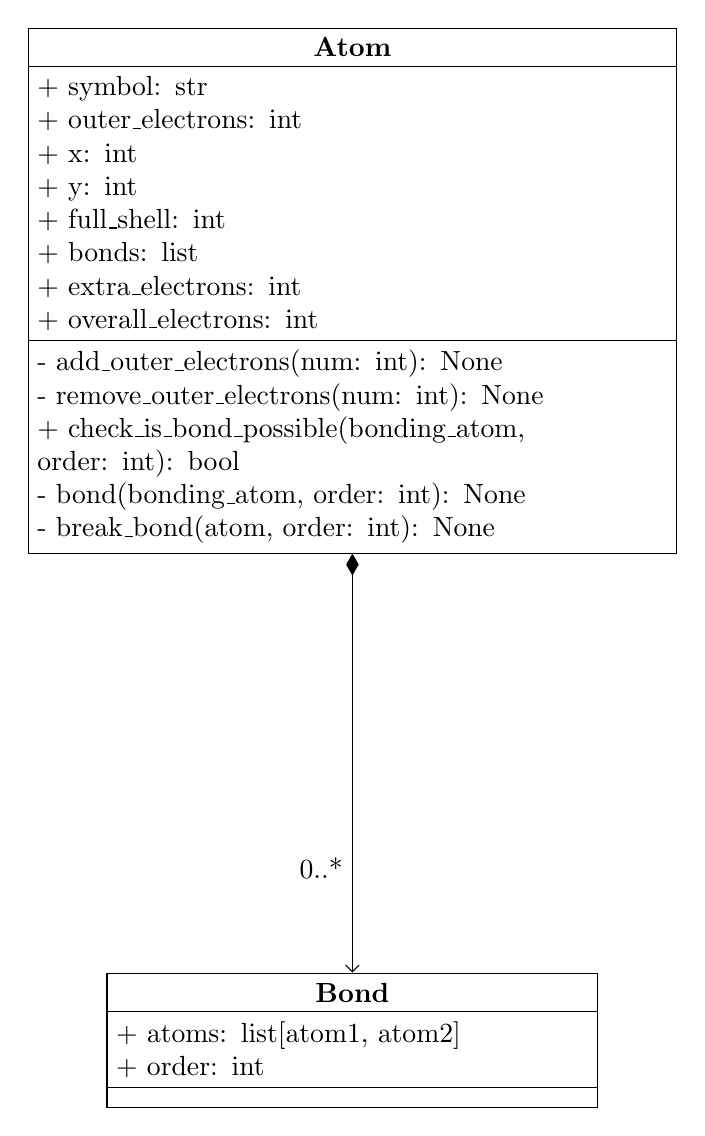
\begin{tikzpicture}
      \begin{class}[text width=8cm]{Atom}{0, 0}
        \attribute{+ symbol: str}
        \attribute{+ outer\_electrons: int}
        \attribute{+ x: int}
        \attribute{+ y: int}
       	\attribute{+ full\_shell: int}
       	\attribute{+ bonds: list}
       	\attribute{+ extra\_electrons: int}
       	\attribute{+ overall\_electrons: int}
        \operation{- add\_outer\_electrons(num: int): None}
        \operation{- remove\_outer\_electrons(num: int): None}
        \operation{+ check\_is\_bond\_possible(bonding\_atom, order: int): bool}
        \operation{- bond(bonding\_atom, order: int): None}
        \operation{- break\_bond(atom, order: int): None}
      \end{class}
      
      \begin{class}[text width=6cm]{Bond}{0, -12}
        \attribute{+ atoms: list[atom1, atom2]}
        \attribute{+ order: int}
      \end{class}
      
      \composition{Atom}{}{0..*}{Bond}
\end{tikzpicture}
\end{center}

\begin{algorithm}
\footnotesize
\caption{Algorithm to check whether a bond is possible}\label{alg:bond_possible}
\begin{algorithmic}
\Function{$check\_is\_bond\_possible$}{$bonding\_atom,\ order$}
\If{$ (overall\_electrons + order) > full\_shell$}
	\State $ RETURN\ False$
\ElsIf{$ (bonding\_atom.overall\_electrons) > bonding\_atom.full\_shell$}
	\State $ RETURN\ False$
\Else 
	\State $ RETURN\ True$
\EndIf
\EndFunction
\end{algorithmic}
\end{algorithm}

Algorithm \ref{alg:bond_possible} investigates whether the suggested bond is chemically possible by using selection statements. The first "if statement" tests if the overall amount of (outer shell) electrons after addition of the extra electron, or electrons dependent on the chosen bond order, it would gain after bonding is greater than the allowed full shell capacity of the atom. If this applies, the subroutine returns the boolean value "False". The subsequent "else if statement" test the exact same thing for the other bonding atom, and returns False if it applies as well. If the program flow manages to get through both of these statements, the method returns "True", as the formation of a bond between the two atoms is possible.

\begin{algorithm}
\footnotesize
\caption{Algorithm for bonding two atoms}\label{alg:bond}
\begin{algorithmic}
\Function{$bond$}{$bonding\_atom,\ order$}
\If{$ check\_is\_bond\_possible = False$}
	\State $ RETURN$
\EndIf
\State $ new\_bond\gets Bond(bonding\_atom,\ order)$
\State $ bonds.append(new\_bond)$
\State $ bonding\_atom.bonds.append(new\_bond)$
\State $ extra\_electrons\gets extra\_electrons + order$
\State $ bonding\_atom.extra\_electrons\gets bonding\_atom.extra\_electrons + order$
\State $ overall\_electrons\gets outer\_electrons + extra\_electrons$
\State $ bonding\_atom.overall\_electrons\gets bonding\_atom.outer\_electrons + bonding\_atom.extra\_electrons$
\EndFunction
\end{algorithmic}
\end{algorithm}

The bonding algorithm (Algorithm \ref{alg:bond}) of the atom class is called when the user wants to bond two atoms together. The opening action of the method uses the subroutine shown in algorithm \ref{alg:bond_possible} to find out if the bond is possible and returns back to the main program is this is not the case. If the check returned a boolean value of "True", a new instance of the class Bond with the correct bond order is created. The freshly formed bond instance is then appended to the list of bonds of each atom, and the number of extra electrons and outer electrons of both atoms is adjusted using the bond order, to correctly store the current amount of electrons each atom has in its outer shell.

\newpage

\subsubsection{ChemEditor GUI}

One issue I encountered early on when working on the canvas was, that the bonds between atoms would start at the centre of the atoms, and it could be complicated to correctly adjust the starting end endpoints of each bond (Figure \ref{fig:atom_bond_overlap}).

\begin{figure} [h]
	\centering
	\includegraphics[scale=0.5]{atom_bond_overlap}
	\caption{Overlap between atoms and bonds}
	\label{fig:atom_bond_overlap}
\end{figure}

To overcome this problem, I decided to create a method for drawing an invisible circle in the same colour as the background behind the symbol of each atom to hide the bonds (draw\_atom\_circle() in code). This method is called after the bonds are drawn, in order to make the overlap with the atoms invisible in the eyes of the user. After drawing the bonds and drawing the circle, the actual atom is drawn on top of it, without any visible overlap between atoms and bonds. Evidently, there is a clear hierarchy as to how the drawing of atoms, bonds and everything else is drawn. After applying the required hierarchy, this is what the bonding of atoms looks like in the current version (Figure \ref{fig:bonds_no_overlap}).

\begin{figure} [h]
	\centering
	\includegraphics[scale=0.5]{bonds_no_overlap}
	\caption{No overlap between atoms and bonds}
	\label{fig:bonds_no_overlap}
\end{figure}

One feature, which I thought would improve the user experience a lot was what I have called "drawing potential bonds". The goal of this is to draw a range of potential atoms and bonds in a circle around the selected atom in a different colour, so that the user only has to click on one of those potential atoms, and it gets drawn as an actual atom with a real bond to the selected atom. The "potential atoms" and the "potential bonds" are related to the element chosen by the user in the "periodic table" and to the buttons suggesting the bond order. To get all the potential positions for the atoms, I created the "calc\_potential\_positions()" subroutine, which takes the atom instance selected by the user as a parameter and then accesses the atoms x and y coordinates and creates an empty list, which will later hold the positions of potential atoms. Using a for loop, the method calculates the x and y vector components using the given angle and magnitude (distance). This subroutine calculates the positions of potential atoms every 45 degrees, and therefore return a maximum of 8 different tuples holding the positions.

\begin{algorithm}
\footnotesize
\caption{Algorithm for finding potential atom positions}\label{alg:calc_potential_pos}
\begin{algorithmic}
\Function{$calc\_potential\_positions$}{$atom$}
\State $ x\gets atom.x\_coords$
\State $ y\gets atom.y\_coords$
\State $ distance\gets 40$
\State $ coordinate\_list\gets NONE$
\For{$ angle\_degrees\gets 0\ TO\ 360\ STEP\ 45$}
	\State $ angle\_radians\gets math.radians(angle\_degrees)$
	\State $ new\_x\gets x\ +\ distance\ *\ math.cos(angle\_radians)$
	\State $ new\_y\gets y\ +\ distance\ *\ math.sin(angle\_radians)$
	\State $ APPEND\ (new\_x,\ new\_y)\ TO\ coordinate\_list$
\EndFor
\State $ RETURN\ coordinate\_list$
\EndFunction
\end{algorithmic}
\end{algorithm}

All the drawing happens in the "paintEvent" method inside the "Canvas" class. To get a better understanding of the following pseudocode for this method, I have put together a table containing all the methods used for it (Table \ref{tab:paintevent_methods}).

\begin{table}[htbp]
    \centering
    \begin{tabularx}{\textwidth}{|X|X|X|}
        \hline
        \textbf{Method Name} & \textbf{Parameters} & \textbf{Description}\\
        \hline
        calc\_potential\_positions & Instance of atom class & Calculates and returns a list of positions for potential atoms in a circle around the atom. \\
        \hline
        check\_atom\_overlap & pos\_x, pos\_y & Iterates through list of atoms and checks for overlap, returns a boolean value. \\
        \hline
        draw\_single\_bond & atom1\_x: int, atom1\_y: int, atom2\_x: int, atom2\_y: int, painter, pen, actual\_bond: bool & Draws a bond line from one atom to another. \\
        \hline
        draw\_double\_bond & atom1\_x: int, atom1\_y: int, atom2\_x: int, atom2\_y: int, painter, pen, actual\_bond: bool & Draws two bond line next to each other from one atom to another. \\
        \hline
        draw\_triple\_bond & atom1\_x: int, atom1\_y: int, atom2\_x: int, atom2\_y: int, painter, pen, actual\_bond: bool & Draws three bond line next to each other from one atom to another. \\
        \hline
        \_\_diagonal\_bonds & atom1\_x: int, atom1\_y: int, atom2\_x: int, atom2\_y: int, painter, offset: int, diag\_offset: int & Handles the drawing of the diagonal bonds in double and triple bonds to avoid overlap of lines. \\
        \hline
        draw\_atom\_circle & atom1\_x: int, atom1\_y: int, atom2\_x: int, atom2\_y: int, painter, pen & Draws a circle in the same colour as the background colour to prevent bonds from visually overlapping with atom. \\
        \hline
        draw\_atom & atom1\_x: int, atom1\_y: int, symbol: str, painter, pen, potential: bool & Draws the atom symbol on the screen. \\
        \hline
    \end{tabularx}
    \caption{Method Descriptions}
    \label{tab:paintevent_methods}
\end{table}

\newpage

The pseudocode of my "paintEvent" method shows the clear structure and hierarchy when it comes to drawing out all the atoms and bonds on the canvas. The method can be broken down in to two main parts, the first one just iterates through a list of atoms and draws the atom and the associated bonds. The second part is only called if an atom is currently selected, and it essentially draws out the possible bonds or potential atoms around it.

\begin{algorithm}
\footnotesize
\caption{paintEvent Algorithm, first part}\label{alg:paintevent_first}
\begin{algorithmic}
\Function{$paintEvent$}{$event$}
\For{$ atom\ IN\ atoms\_list$}
	\State $ draw\_atom(x,\ y,\ symbol,\ painter,\ pen,\ False)$
	\For{$ bond\ IN\ atom.bonds$}
		\If{$ bond.order = 2$}
			\State $ draw\_double\_bond(x1,\ y1,\ x2,\ y2,\ symbol,\ painter,\ True)$
		\ElsIf{$ bond.order = 3$}
			\State $ draw\_triple\_bond(x1,\ y1,\ x2,\ y2,\ symbol,\ painter,\ True)$
		\Else
			\State $ draw\_single\_bond(x1,\ y1,\ x2,\ y2,\ symbol,\ painter,\ True)$
		\EndIf
		\State $ draw\_atom\_circle(x2,\ y2,\ x1,\ y1,\ painter,\ pen)$
		\State $ draw\_atom(x2,\ y2,\ symbol2,\ painter,\ pen,\ False)$
		\State $ draw\_atom(x1,\ y1,\ symbol1,\ painter,\ pen,\ False)$
	\EndFor
\EndFor
\State SECOND\ PART\ HERE
\EndFunction
\end{algorithmic}
\end{algorithm}

For visualisation purposes, I have decided to split the pseudo code for the "paintEvent" method into the two parts mentioned before.\\
As explained in an earlier part, it is essential to follow a certain hierarchy structure for drawing out the canvas. Algorithm \ref{alg:paintevent_first} (paintEvent Algorithm, first part) illustrated this procedure perfectly. The very first thing to happen every time the "paintEvent" is called, is that using an iterative for-loop structure, every atom in the atoms list is being drawn on the canvas. In the bigger picture, this is so that all the atoms that are not bonded and don't need anything extra are drawn. Next, all the bonds of the specific atom are displayed, and the "atom circle" is drawn. And lastly both atoms on either side of the bond are drawn and the first part of the "paintEvent" method is completed. As noted at the start of this sub-section 2.6, it is important that for bonded atoms, the bond is drawn first, then the "atom circle" and lastly the actual atoms.

\newpage

\begin{algorithm}
\footnotesize
\caption{paintEvent Algorithm, second part}\label{alg:paintevent_second}
\begin{algorithmic}
\If{$ selected = True$}
	\State $ x1\gets selected\_atom.x\_coords$
	\State $ y1\gets selected\_atom.y\_coords$
	\If{$ action\_type != "bond"$}
		\If{$ selected\_atom\ IS\ NOT\ NONE$}
		\State $ potential\_positions\gets calc\_potential\_positions(selected\_atom)$
		\For{$ pos\ IN\ potential\_positions$}
			\If{$ check\_atom\_overlap(pos[0],\ pos[1]) = False$}
				\If{$ bond\_order = 2$}
					\State $ draw\_double\_bond(x1,\ y1,\ pos[0],\ pos[1],\ painter,\ pen,\ False)$
				\ElsIf{$ bond\_order = 3$}
					\State $ draw\_triple\_bond(x1,\ y1,\ pos[0],\ pos[1],\ painter,\ pen,\ False)$
				\Else
					\State $ draw\_single\_bond(x1,\ y1,\ pos[0],\ pos[1],\ painter,\ pen,\ False)$
				\EndIf
				\State $ draw\_atom\_circle(pos[0],\ pos[1],\ x1,\ y1,\  painter,\ pen)$
				\State $ draw\_atom(pos[0],\ post[1],\ symbol,\ painter,\ pen,\ True)$
				\State $ draw\_atom(x1,\ y1,\ symbol,\ painter,\ pen,\ False)$
			\EndIf
		\EndFor
	\EndIf
	\EndIf
\EndIf
\end{algorithmic}
\end{algorithm}

This second part of the "paintEvent" (Algorithm \ref{alg:paintevent_second}), uses the\\
"calc\_potential\_positions()" method discussed earlier and all in all just puts the whole functionality of drawing potential atoms and bonds around the selected atom together.\\

The "mousePressEvent" subroutine handles the users actions on the canvas. The pseudocode for this algorithm is divided into two separate blocks for visualisation purposes (Algorithm \ref{alg:mousePressEvent_one} and Algorithm \ref{alg:mousePressEvent_two}). The method initially uses "if statements" to find out which action type the user has currently selected (draw, bond, remove). If the selected action type is "remove", the atom at the click position and if applicable all of the atoms bonds are removed.\\

\newpage

\begin{algorithm}
\footnotesize
\caption{mousePressEvent Algorithm, first part}\label{alg:mousePressEvent_one}
\begin{algorithmic}
\Function{$mousePressEvent$}{$event$}
\If{$ user\ clicked\ on\ canvas$}
	\State $ click\_pos\gets user\ click\ position$
	\If{$ action\_type = "remove"$}
		\State $ remove\_bond(click\_pos.x,\ click\_pos.y)$
		\State $ remove\_atom(click\_pos.x,\ click\_pos.y)$
	\ElsIf{$ action\_type = "bond"$}
		\For{$ atom in atoms\_list$}
			\State $ atom\_x\gets atom.x\_coords$
			\State $ atom\_y\gets atom.y\_coords$
			\If{$ atom\ position = click\ position$}
				\State $ selected\gets True$
				\State $ selected\_atom\gets atom$
				\State $ temp\_bond\_list.append(atom)$
				\If{$ LEN(temp\_bond\_list) = 2$}
					\If{$ temp\_bond\_list[0] = temp\_bond\_list[1]$}
						\State $ OUTPUT\ "Trying\ to\ bond\ to\ itself"$
						\State $ temp\_bond\_list.CLEAR()$
						\State $ RETURN$
					\EndIf
					\State $ temp\_bond\_list[0].bond(temp\_bond\_list[1],\ bond\_order)$
					\State $ temp\_bond\_list.CLEAR()$
					\State $ selected\_atom\gets NONE$
				\EndIf
				\State $ RETURN$
			\EndIf
			\State $ selected\gets False$
		\EndFor
	\Else
		\State $ SECOND\ PART\ HERE$
	\EndIf
\EndIf
\EndFunction
\end{algorithmic}
\end{algorithm}

If the user has selected "bond", the program iterates over the list of all atoms on the canvas, and compares each atoms position with the users click position. If the click position matches the coordinates of an atom, this atom is added to a temporary list, and gets bonded to the other atom in that list as soon as the length of this list is equal to two.

\newpage

Lastly, in the second part of the subroutine (Algorithm \ref{alg:mousePressEvent_two}), which can be imagined to be placed in algorithm \ref{alg:mousePressEvent_one} after the last else statement where it says " SECOND PART HERE", if the user has selected the draw action, another selection is used to check whether an atom is currently selected. If this is the case, it means that the circle with potential atoms is currently displayed. This section now evaluates whether the user has clicked on one of the potential atoms and therefore allows this atom and bond to be permanently added to the canvas, and then creates those new atoms and bonds. Otherwise, if the user has not clicked on an atom, this means that they have clicked on a blank area on the canvas, a new atom is created at the click position and added to the list of atoms on the canvas.

\begin{algorithm}
\footnotesize
\caption{mousePressEvent Algorithm, second part}\label{alg:mousePressEvent_two}
\begin{algorithmic}
\If{$ selected = True$}
	\If{$ selected\_atom\ IS\ NOT\ NONE$}
		\State $ potential\_positions\gets calc\_potential\_positions(selected\_atom)$
		\If{$ check\_atom\_overlap(pos) = False$}
			\For{$ pos\ IN\ potential\_positions$}
				\If{$ pos = click position$}
					\State $ new\_atom\gets Atom(element,\ pos)$
					\If{$ new\_atom.check\_is\_bond\_possible(selected\_atom,\ bond\_order) = True$}
						\State $ atoms\_list.append(new\_atom)$
						\State $ new\_atom.bond(selected\_atom,\ bond\_order)$
					\EndIf
				\EndIf
			\EndFor
			\State $ selected\gets False$
		\EndIf
	\EndIf
\EndIf
\If{$ check\_clicked\_on\_atom(pos) = True$}
	\State $ RETURN$
\EndIf
\State $ new\_atom\gets Atom(element,\ pos)$
\State $ atoms\_list.append(new\_atom)$
\end{algorithmic}
\end{algorithm}

\newpage

\section{Testing}

As usual with software projects, a lot of undocumented exploratory testing is happening during the production phase. A good example for this would be the tests shown in Figure \ref{fig:initial_balance_test}, \ref{fig:second_balance_test} and \ref{fig:working_balancer}, which luckily got captured in the moment.

\subsubsection{Tests for ChemCalculator}

The following tables contain an overview of basic input and output tests on the ChemCalculator module to ensure that the expected outcomes align with the actual outcomes during system usage. As this module has many very similar features, I have decided to summarise those tests into fewer fields, to make this section less repetitive. The tests will of course still contain any outliers of the testing process.

\begin{table}[htbp]
\centering
\begin{tabularx}{\textwidth}{|p{1cm}|X|X|X|X|}
\hline
\textbf{Test No.} & \textbf{Description} & \textbf{TEX (Typical, Erroneous, Extreme} & \textbf{Expected Outcome} & \textbf{Actual Outcome} \\
\hline
\multirow{3}{*}{1} & Calculate value for blank input & T: Fill 2 out of 3 input options with common values & Blank field calculated correctly. & As expected.\\
\cline{3-5}
& & E: Fill in all 3 input options with common values & Must leave exactly one input line empty for it to be calculated! & As expected.\\
\cline{3-5}
& & X: Use invalid characters & Only numerical values in the form of integers or decimals allowed! & As expected.\\

\hline

\multirow{3}{*}{2} & Test unit drop down  & T: Change units & Value scales accordingly. & As expected.\\

\hline
\end{tabularx}
\caption{Universal Calculator tests}
\label{tab:calculator_tests}
\end{table}

\begin{table}[htbp]
\centering
\begin{tabularx}{\textwidth}{|p{1cm}|X|X|X|X|}
\hline
\textbf{Test No.} & \textbf{Description} & \textbf{TEX (Typical, Erroneous, Extreme} & \textbf{Expected Outcome} & \textbf{Actual Outcome} \\
\hline
\multirow{3}{*}{3} & Calculate value for blank input & T: Leave one input blank & Blank field calculated correctly. & As expected.\\
\cline{3-5}
& & E: Fill in all input options with common values & Must leave one input line empty for it to be calculated! & As expected.\\
\cline{3-5}
& & X: Use invalid characters & Only numerical values in the form of integers or decimals allowed! & As expected.\\

\hline
\multirow{3}{*}{4} & Calculate value for multiple blank inputs & T: Leave allowed combination of inputs blank & Blank fields calculated correctly. & Must leave one input line empty for it to be calculated!\\
\cline{3-5}
& & E: Leave two critical inputs blank (mass and molecular weight) & Must leave one input line empty for it to be calculated! & As expected.\\
\hline
\end{tabularx}
\caption{Avogadro's constant calculator tests}
\label{tab:avogadros_tests}
\end{table}

Table \ref{tab: avogadros_tests} shows the only outlier out of all the tests conducted on the ChemCalculator module. The Avogadro's calculator can with certain combinations of inputs also work with two blank inputs. The outlier can be found in the typical (T) row of test no. 4, where allowed combinations of empty inputs are tested. Allowed combinations in this case would be leaving the "mass" and the "number of atoms" lines blank, as the "number of atoms" input can be calculated from the combination of the moles and Avogadro's constant and calculating the mass only requires the molecular weight and the moles.\\
To correct this, I have used "if-statements" to find out which line have been left blank and which ones have not. After applying this in a correct sequence and implementing our error dialogue, the calculator now works in the expected way and produces the desired output.

\subsubsection{Tests for ChemBalancer}

To test the robustness and efficiency of the balancer, I chose to pick an independent list of chemical equations to find out if my program can handle every different type of equation listed.
The following chemical equations represent a sample of the tests for robustness and efficiency applied on the balancer. This list was published as a part of an article on "Journal of High School Science". Note that the equations are not written with proper subscript formatting, as it is shown in the format, which the balancer takes as an input and produces as an output, with the only difference, that arrows are used here compared to equals signs in the program.

\begin{enumerate}

\item Unbalanced equation: C4H10 + O2 → CO2 + H2O\\ Balanced equation: 2C4H10 + 13O2 → 8CO2 + 10H2O

\item Unbalanced equation: (NH4)2Cr2O7 → N2 + Cr2O3 + H2O\\ Balanced equation: (NH4)2Cr2O7 → N2 + Cr2O3 + 4H2O

\item Unbalanced equation: C57H110O6 + O2 → CO2 + H2O\\ Balanced equation: 2C57H110O6 + 163O2 → 114CO2 + 110H2O

\item Unbalanced equation: KNO3 + C12H22O11 → N2 + CO2 + H2O + K2CO3\\ Balanced equation: 48KNO3 + 5C12H22O11 → 24N2 + 36CO2 + 55H2O + 24K2CO3

\item Unbalanced equation: Cu2S + HNO3 → Cu(NO3)2 + CuSO4 + NO2 + H2O\\ Balanced equation: 1Cu2S + 12HNO3 → 1Cu(NO3)2 + 1CuSO4 + 10NO2 + 6H2O

\item Unbalanced equation: K4[Fe(SCN)6] + K2Cr2O7 + H2SO4 → Fe2(SO4)3 + Cr2(SO4)3 + CO2 + H2O + K2SO4 + KNO3\\ Balanced equation: 6K4[Fe(SCN)6] + 97K2Cr2O7 + 355H2SO4 → 3Fe2(SO4)3 + 97Cr2(SO4)3 + 36CO2 + 355H2O + 91K2SO4 + 36KNO3

\item Unbalanced equation: Na2S2O4 + NaOH → Na2SO3 + Na2S + H2O\\ Balanced equation: 3Na2S2O4 + 6NaOH → 5Na2SO3 + 1Na2S + 3H2O

\item Unbalanced equation: C6H8O7 + NaHCO3 → Na3C6H6O7 + CO2 + H2O\\ Balanced equation: 19C6H8O7 + 54NaHCO3 → 18Na3C6H6O7 + 60CO2 + 49H2O

\item Unbalanced equation: P4O10 + H2O → H3PO4\\ Balanced equation: 1P4O10 + 6H2O → 4H3PO4

\end{enumerate}

While conducting these tests, an unexpected issue appeared, where if an invalid equation is given, with an arrow instead of an equals sign for example (I.e.: C4H10 + O2 → CO2 + H2O instead of C4H10 + O2 = CO2 + H2O),the program has first opened a dialogue stating the issue to the user and then after the arrow has been changed to an equals sign, the application crashed upon hitting the "balance" button. Figure \ref{fig:balancer_crash} shows the crash report for this bug. 

\begin{figure} [h]
	\centering
	\includegraphics[scale=0.3]{balancer_crash}
	\caption{Balancer Crash Report}
	\label{fig:balancer_crash}
\end{figure}

I have resolved this issue using pythons exception handling. As the ChemBalancer module has many methods calling other methods, I have had to nest every relevant method in a try - except statement and raise this exception to the next higher method level. A smaller example version this solution is shown in Listing \ref{lst:balancer_exceptions}.

\begin{lstlisting}[language=Python, caption=Example of exception structure, label={lst:balancer_exceptions}]
def lowest_level_function():
	try:
	    # Do something...
    except Exception:
	    raise # Raise the exception to be caught by the next higher level function

def middle_level_function():
    try:
        lowest_level_function()
    except Exception:
        raise  # Re-raise the exception to be caught by the highest level function

def highest_level_function():
    try:
        middle_level_function()
    except Exception:
        return  # Stop further execution of highest level function
\end{lstlisting}

After eliminating the mentioned issues, I have tested the program with the entries of the list of equations again. The balancer has successfully produced the desired balanced equation every time. An example of a chemical equation balanced by the ChemBalancer is given in Figure \ref{fig:final_balancer_test}. For this example I chose equation number 6 from the list, as this shows a very complex chemical equation that would be incredibly hard for a human to balance without any tools, which is exactly what the purpose of this project is.

\begin{figure} [h]
	\centering
	\includegraphics[scale=0.3]{final_balancer_test}
	\caption{Working test of balancer}
	\label{fig:final_balancer_test}
\end{figure}

\subsubsection{Tests for ChemEditor}

As with the other modules, most features were tested by exploratory test during development. I have tried to summarise the tests for the ChemEditor in the following table.

\begin{table}[htbp]
\centering
\begin{tabularx}{\textwidth}{|p{1cm}|X|X|X|X|}
\hline
\textbf{Test No.} & \textbf{Description} & \textbf{TEX (Typical, Erroneous, Extreme} & \textbf{Expected Outcome} & \textbf{Actual Outcome} \\
\hline
\multirow{3}{*}{1} & Draw atoms & T: Click on a blank are on the canvas & Atom gets drawn at click position. & As expected.\\

\hline

\multirow{3}{*}{2} & Bond two atoms together & T: Select bond action type and click on two different atoms & Bond between atoms appears. & As expected\\
\cline{3-5}
& & E: Click on at least one atom with full or near full outer shell with high bond order so that overall electrons would be greater than the full shell & Invalid user Action! & As expected.\\
\cline{3-5}
& & X: Select bond action type and click on the same atom twice & Invalid user Action! & As expected.\\
\hline

\multirow{3}{*}{3} & Remove Atom & T: Select remove action type and click on atom & Atom and connected bonds disappear & As expected\\

\hline

\end{tabularx}
\caption{ChemEditor tests}
\label{tab:editor_tests}
\end{table}


\newpage

\section{Evaluation}

The following tables compare the finished system with the set objectives at the beginning of this document.

Colour keys for comparison:

\begin{table}[htbp]
\footnotesize
\centering
\begin{tabularx}{\textwidth}{|X|X|X|X|}

\hline
\cellcolor{red!70} Objective not met & \cellcolor{orange!70} Objective partially met & \cellcolor{cyan!70} Objective met & \cellcolor{green!70} Objective exceeded\\
\hline

\end{tabularx}
\label{tab:color_keys}
\end{table}

\subsubsection{Objective Comparison for ChemCalculator}

\begin{table}[htbp]
\centering
\begin{tabularx}{\textwidth}{|X|X|}
\hline
\textbf{Original Objective} & \textbf{Completed System}\\

\hline

Standard moles calculator & \cellcolor{cyan!70} Objective met. \\

\hline

Concentration calculator & \cellcolor{cyan!70} Objective met. \\

\hline

Avogadro's number calculator with included moles calculator (mass/molar mass) & \cellcolor{cyan!70} Objective met. \\

\hline

Gibbs Free Energy calculator & \cellcolor{cyan!70} Objective met. \\

\hline

Specific heat capacity calculator & \cellcolor{cyan!70} Objective met. \\

\hline

Equilibrium constant calculator & \cellcolor{cyan!70} Objective met. \\

\hline

Rate calculator calculator & \cellcolor{cyan!70} Objective met. \\

\hline

Ideal Gas Law calculator & \cellcolor{cyan!70} Objective met. \\

\hline

\end{tabularx}
\caption{ChemCalculator objective comparison}
\label{tab:calc_objective_comp}
\end{table}

\subsubsection{Objective Comparison for ChemBalancer}

\begin{enumerate}

\item Handling Brackets: The balancer appropriately deals with chemical equations containing brackets. It uses regular expressions to recognise and process substances enclosed within brackets and correctly identifies separate reagents and elements.

\item Support for subscript numbers: Subscript numbers are identified correctly in the unbalanced equation and are handled in a way that the equation can be balanced properly.

\item Support for complex ions: Although the balancer can easily deal with equations containing square brackets ([ ]), it can not yet handle ionic charges. So the balancer can deal with chemical equations in the form of complex ions as long as charges are not included.

\item Handling complex unbalanced equations: The system successfully handles long and complex user inputs, and correctly identifies individual reagents, elements, brackets and subscripts.

\item Conversion to balanced equations: The ChemBalancer accurately converts unbalanced chemical equations into balanced versions, providing the user has followed the allowed "syntax" and rules for the module. It applies the necessary coefficients to each compound to ensure that the number of atoms of each element is equal on each side of the equation.

\end{enumerate}

In summary, the ChemBalancer module successfully meets most of the set objectives, with the exception of complex ions. The system demonstrates its capability to balance most equations effectively, and it serves its purpose well.

\subsubsection{Objective Comparison for ChemEditor}

\begin{table}[htbp]
\centering
\begin{tabularx}{\textwidth}{|X|X|}
\hline
\textbf{Original Objective} & \textbf{Completed System}\\

\hline

Provide a user-friendly and easy to use interface. & \cellcolor{cyan!70} The finished system has a very easy to use interface including pop-up dialogues for invalid user actions. \\

\hline

Have a range of commonly used elements for the user to choose from. & \cellcolor{green!70} The ChemEditor provides the user with a near full periodic table including all the period 1, 2, 3, 4 and 5 elements. \\

\hline

Support ions and let the user choose different charges on atoms (ions) & \cellcolor{red!70} This module does not yet support ions. \\

\hline

Allow for single, double and triple bonds & \cellcolor{cyan!70} The user can choose between different bond orders. \\

\hline

Conduct real-time checks to ensure atoms do not exceed their valence electrons.  & \cellcolor{cyan!70} The program stores the elements valence electrons and checks if a new bond would lead to a higher number of electrons in the outer shell than allowed every time the user tries to bond two atoms together. \\

\hline


\end{tabularx}
\caption{ChemEditor objective comparison}
\label{tab:editor_objective_comp}
\end{table}

\begin{table}[htbp]
\centering
\begin{tabularx}{\textwidth}{|X|X|}
\hline
\textbf{Original Objective} & \textbf{Completed System}\\

\hline

Tool bar containing buttons for the choice of element and bond order  as well as options for choosing different action types like bond, draw or remove. & \cellcolor{green!70} The tool contains the option for opening the periodic table, choose the preferred bond order, action types like bond, draw and remove, as well as giving the option to clear the canvas or save it as an image. \\

\hline

Draw atoms at click position on canvas & \cellcolor{cyan!70} The system draws an atom of the chosen element at the user's click position. \\

\hline

Display a number of potential atoms and bonds when the user clicks on existing atom in draw mode. & \cellcolor{cyan!70} System draws up to 8 potential atoms and bonds in a circle around the selected atom. \\

\hline

Provide the ability to bond atoms together & \cellcolor{cyan!70} The system bonds the two latest selected atoms together \\

\hline

\end{tabularx}
\caption{ChemEditor objective comparison}
\label{tab:editor_objective_comp2}
\end{table}

\subsubsection{Potential for Future Development}

Thanks to the nature of the project, there are always new tools or features one could add. If the project were to be revisited in the future, the first task might be to include the non-essential objectives in the system. Also, two great features to add would be the accepting ionic charges in the balancer and being able to draw ions (with charges) on the canvas of the ChemEditor.\\
As the field of chemistry is very broad, and even physicists could find use in a all-in-one toolbox, there is an unlimited range of possible future additions when it comes to new calculations or new drawing methods like drawing 3D molecules. As this program was created as an A-Level project, it doesn't even come close to the features required by an undergraduate or postgraduate student, so this could be picked up again at a later stage to add required features by those kinds of users.\\ 
A project like this would be a great open source software, where students and scientists from all over the world and every kind of level of education could add features they might require or know to be required by other people.

\subsubsection{User Feedback}

\begin{figure}[H]
	\centering
	\includegraphics[scale=0.8]{UserFeedback}
	\label{fig:user_feedback}
\end{figure}

\newpage

\printbibliography[heading=bibintoc]

\newpage
\begin{appendices}

\section{Program Code}

\subsection{main.py File}

\lstinputlisting[language=Python, caption=main.py File Program Code, label={lst:main_file}]{main.py}


\subsection{GUI Components File}

\lstinputlisting[language=Python, caption=gui\_comps.py File Program Code, label={lst:gui_comps_file}]{gui_comps.py}


\newpage

\subsection{ChemCalculator File}
\input{sections/CalculatorCode}

\newpage

\subsection{ChemBalancer File}

\lstinputlisting[language=Python, caption=chem\_balancer.py File Program Code, label={lst:chem_balancer_file}]{chem_balancer.py}

\newpage

\subsection{ChemEditor GUI file}

\lstinputlisting[language=Python, caption=chem\_editor\_gui.py File Program Code, label={lst:chem_editor_gui_file}]{chem_editor_gui.py}

\newpage

\subsection{ChemEditor Logic file}

\lstinputlisting[language=Python, caption=chem\_editor\_logic.py File Program Code, label={lst:chem_editor_logic_file}]{chem_editor_logic.py}

\newpage

\subsection{Style.css file}

\lstinputlisting{style.css}

\newpage

\subsection{Elements.json file}

\lstinputlisting{elements.json}

\end{appendices}



\end{document}
